\section{Application-Specific RunTime Manager}


\begin{figure}
	\centering
	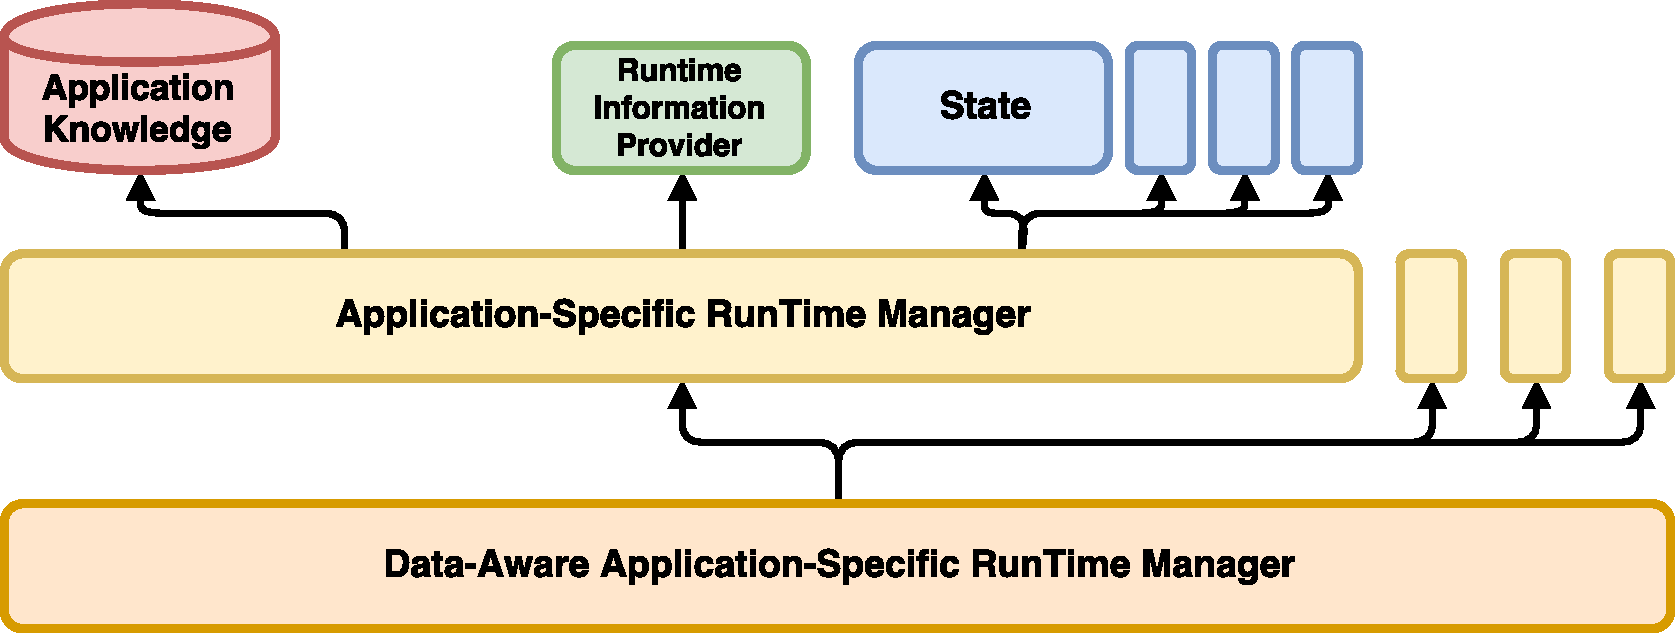
\includegraphics[scale=0.5]{asrtm}
	\caption{Overview of the manager module. }
	\label{fig:asrtm_module}
\end{figure}


This section describes the heart of mARGOt: the Manager module.
This module is in charge of selecting the most suitable configuration for the application.
\prettyref{fig:asrtm_module} shows the overall architecture of the module and the interaction between its principal elements.
In the remainder of the section, each element is explained in more details, following a bottom up approach.
However, the application developer has to interact only with the Application-Specific RunTime Manager (ASRTM) element or with the Data-Aware Application-Specific RunTime Manager element (DA-ASRTM).


\subsection{Rutime Information Provider}

This element relates the expected behavior of the application, in terms of EFPs, with the ones observed by the monitors.
In particular, since the framework will provide to the application a configuration which belong to the application knowledge, mARGOt knows the expected behavior of the application.
Therefore, if there is some difference between the expected behavior and the actual behavior of the application, the idea is that the framework must adjust the application knowledge accordingly.
To achieve this goal, the runtime information manage define the \textbf{coefficient error} $c_{e}^{i}$ for the \textit{i-th} field of the Operating Point as reported in \prettyref{eq:coefficient_error}.

\begin{equation}
\label{eq:coefficient_error}
c_{e}^{i}=\dfrac{expected_{i}}{mean_{i}}
\end{equation}

Where $mean_{i}$ represents the mean value observed by the related monitor and $expected_{i}$ represents the expected value, contained in the application knowledge.
Therefore, if $c_{e}^{i}$ is equal to $1$, it means that the $i-th$ field of the application knowledge matches perfectly with information provided by the monitor.
For numerical stability, if the observed value of the metric is exactly equal to zero, the framework adds a padding value of $1$ to the numerator and to the denominator.
In this case, $c_{e}^{i}$ tends to underestimate the actual value.

Typically, each measured value is affected by noise, produced either by the operating system or by the technique used to gather the measure.
To be robust with respect to this kind of noise, if the mean value observed by the monitor is within one standard deviation with respect to the expected mean value, we set $c_{e}^{i}$ equal to one.
The latter scenario requires that the target field is defined as a distribution in the application knowledge.
The idea is to adapt only if the difference is statistically significant.

Since some metrics may have spikes due to exceptional events, for instance when a process is migrated to another computing element, the runtime information provider store the last $n$ $c_{e}^{i}$ in a circular buffer, initially filled with ones (we assume that the application knowledge matches the reality).
The framework names \textbf{inertia} the value $n$.
If we set an high inertia to the \textit{i-th} field of an Operating Point, we are less prune to react over extraordinary events, but we are also less responsive in case of abrupt changes on the application behavior.
This parameter is exposed to the end user.


Therefore, the actual coefficient error used by the framework $\bar{c_{e}^{i}}$ is the average of all the $c_{e}^{i}$ gathered at runtime, as defined in \prettyref{eq:coefficient_error_real}.
Where $j$ indicates the \textit{j-th} $c_{e}^{i}$ in the circular buffer and $n$ indicates the inertia of the \textit{i-th} field.


\begin{equation}
\label{eq:coefficient_error_real}
\bar{c_{e}^{i}}=\dfrac{\sum_{j=0}^{n-1} c_{e,j}^{i}}{n}
\end{equation}


mARGOt uses $\bar{c_{e}^{i}}$ to perform a linear error propagation.
For examples, if with the selected configuration we expect a throughput of $10fps$, but the throughput monitor observe a throughput of $8fps$, mARGOt assumes that also all the other Operating Points will have a throughput that is $20\%$ slower than expected.
Since the error coefficient for the $i-th$ field of the Operating Point is computed in an independent way from the error coefficient of the $j-th$ field, mARGOt is able to perform a fine grained scaling of the application knowledge, to face changes in the execution environment.


